\subsection{19 августа. Д.р. Кичкинакол Уллукёльский}

Подъём дежурных в 05:00, общий подъём в 05:30 \remove{под бодрую еврейскую песню на гуслях <<Ломирр зих ибербетн>>.~ }
Выходим в 07:30, идём по 

\begin{figure}[h]
	\centering
	\includegraphics[width=0.7\linewidth]{../pics/DSC_0658}
	\caption{Группа в верховьях д.р. Кичкинакол Уллукёльский}
	\label{fig:DSC_0658}
\end{figure}

\begin{figure}[h]
	\centering
	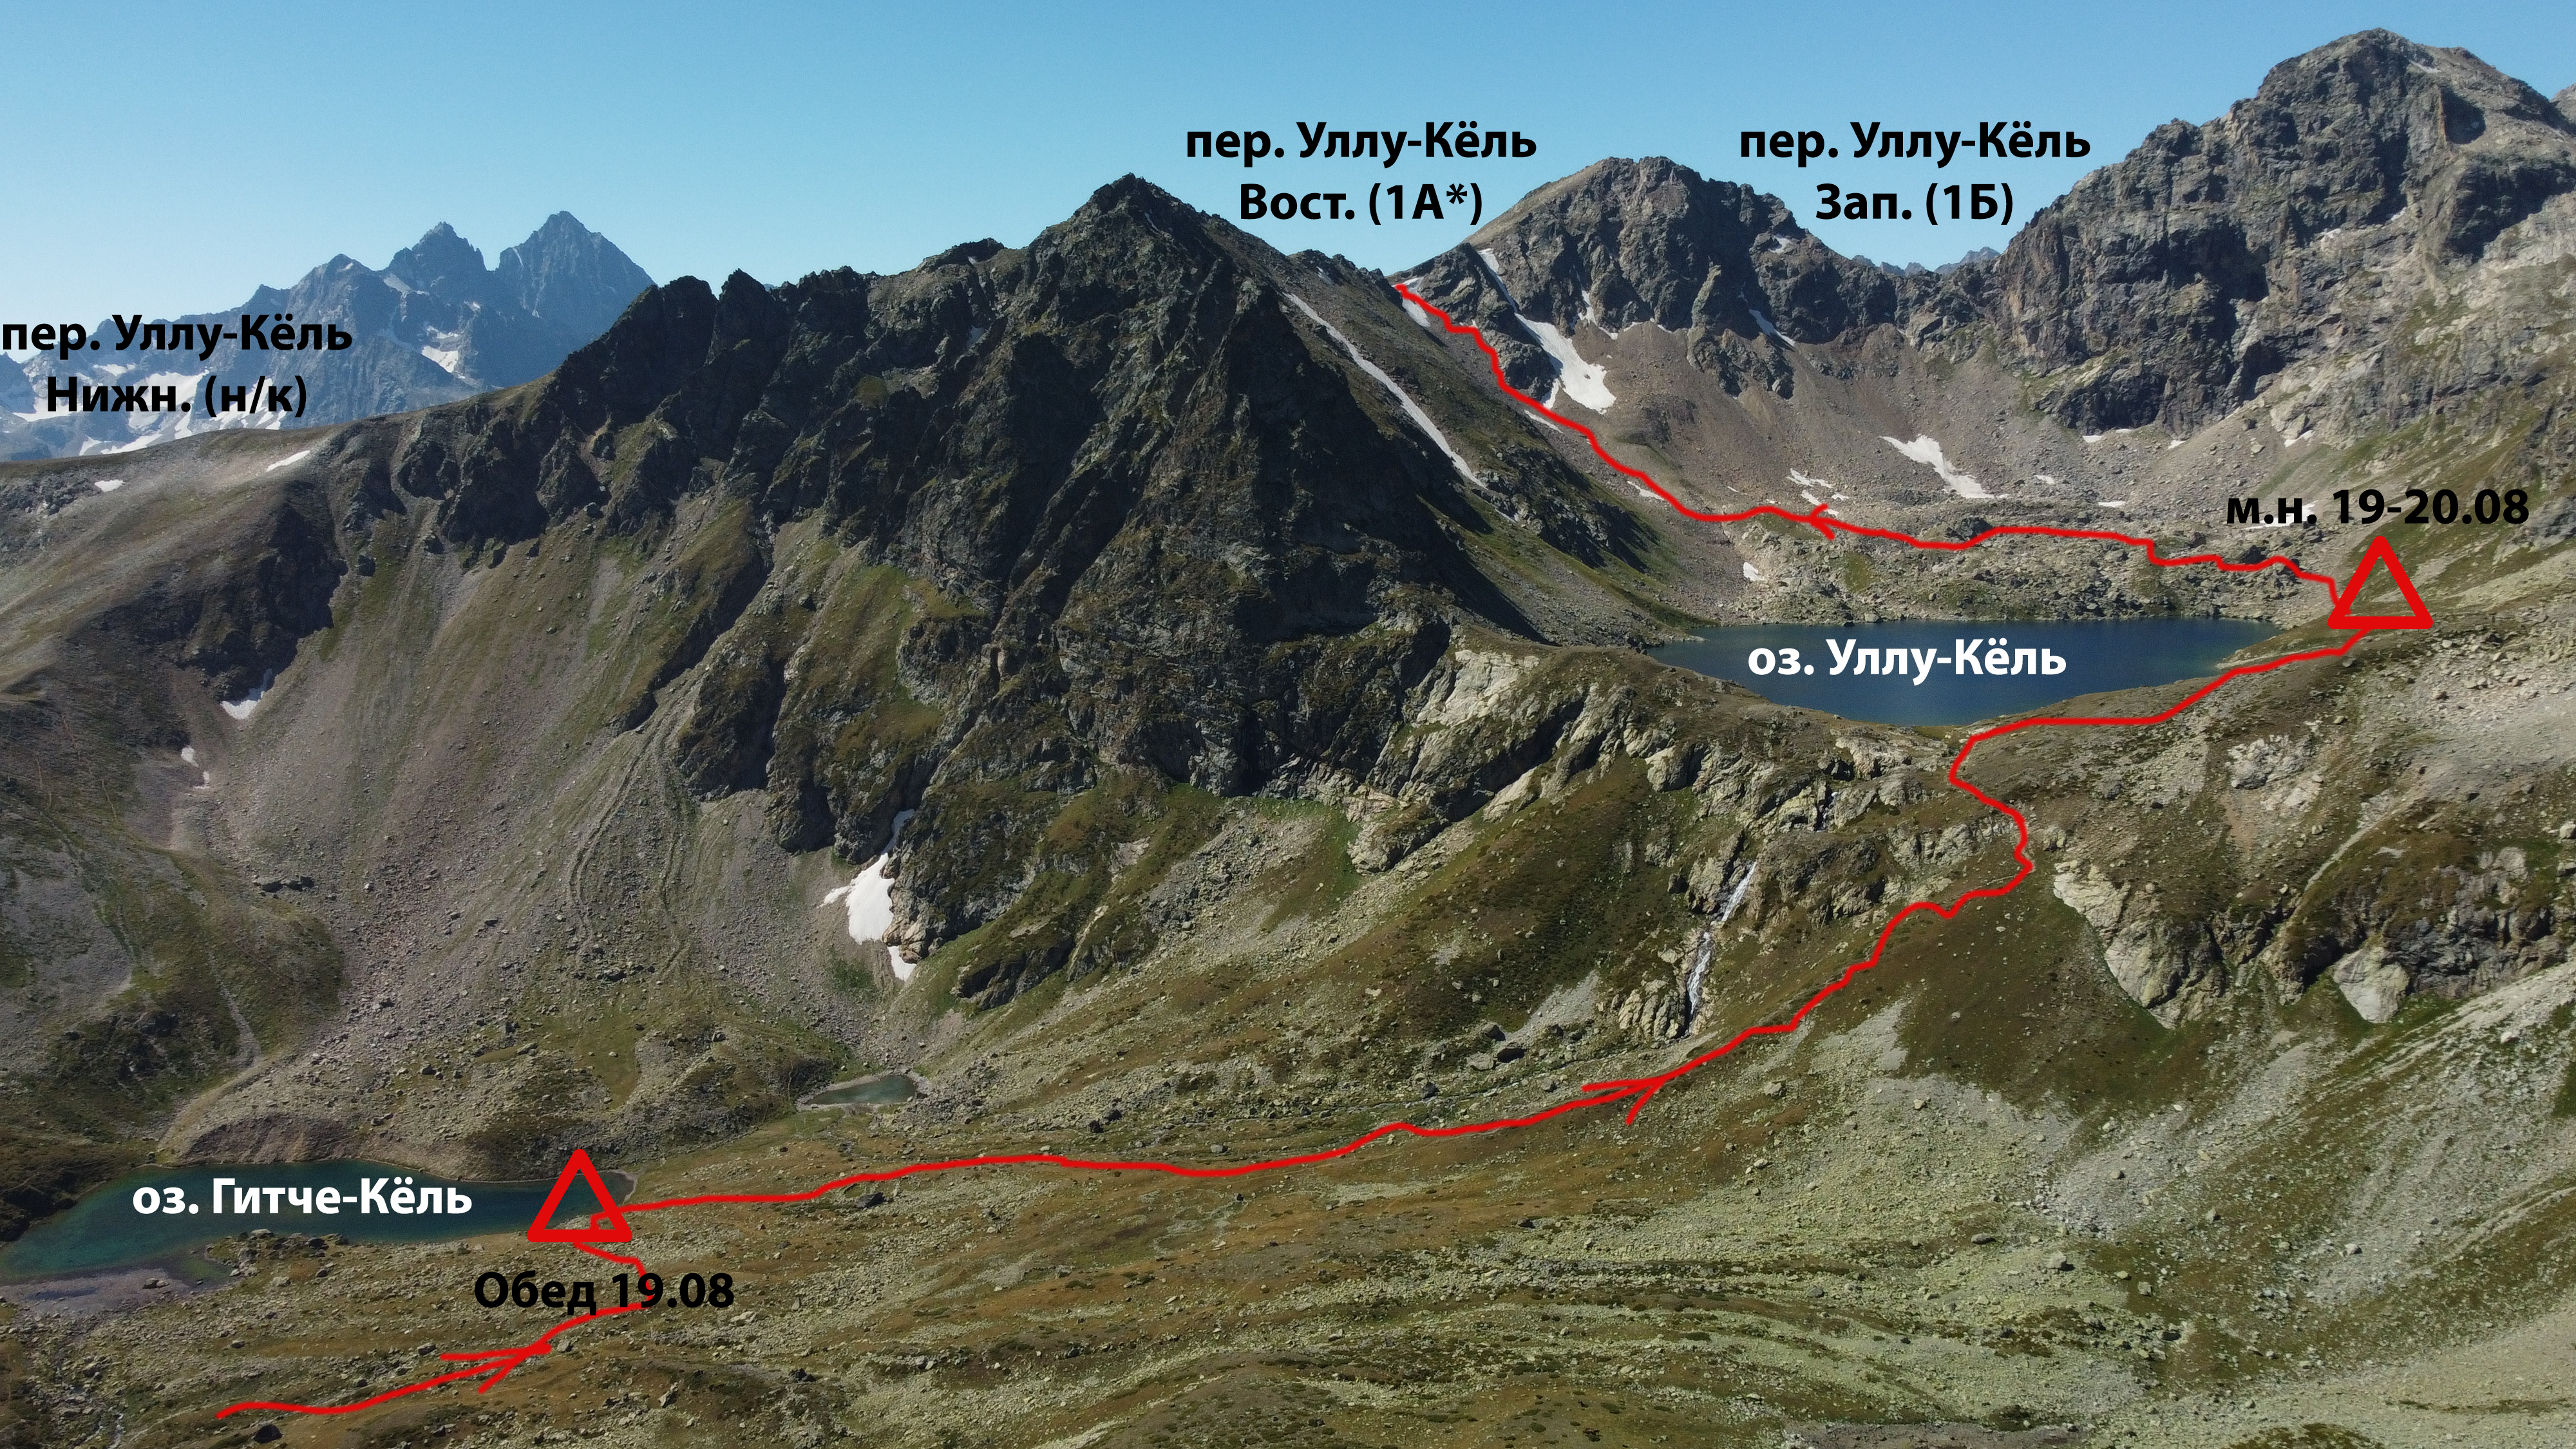
\includegraphics[width=0.7\linewidth]{../pics/ullu_kuel_route}
	\caption{Дорога до озёр и далее на перевал}
	\label{fig:ullu_kuel_route}
\end{figure}

\begin{figure}[h]
	\centering
	\begin{turn}{90}
		\includegraphics[width=0.7\linewidth]{../pics/DSC_0774}
	\end{turn}
	\caption{Купаемся в оз. Гитче-Кёль}
	\label{fig:DSC_0774}
\end{figure}

\begin{figure}[h]
	\centering
	\includegraphics[width=0.7\linewidth]{../pics/DSC_0800}
	\caption{Группа на оз. Уллу-Кёль}
	\label{fig:DSC_0800}
\end{figure}

\newpage